\chapter{Yhtälö}

Monissa käytännön tilanteissa jokin suure voidaan päätellä tai laskea kahdella eri tavalla. Nämä tavat voidaan merkitä lukuina tai kirjoittaa lausekkeiksi. Merkitsemällä näin saadut lukuarvot ja lausekkeet yhtäsuuriksi saadaan \emph{yhtälö}. Yhtälö on siis kahden lausekkeen merkitty yhtäsuuruus. Yhtälöitä esiintyy usein käytännön tilanteissa.

\begin{esimerkki}
Merkitään lausekkeet $5x+\sqrt{x}$ ja $7x+7$ yhtäsuuriksi, jolloin saadaan
yhtälö $5x+\sqrt{x} = 7x+7$.
\end{esimerkki}

\laatikko{
Jos yhtälön kummankin puolen lausekkeen arvo on sama, sanotaan että \emph{yhtälö pätee}.
}

\begin{esimerkki}
\begin{enumerate}[a)]
\item Yhtälö $3x + 2 = 0$ pätee, kun $x = - \frac{2}{3}$.
\item Yhtälö $5 = 3$ ei päde.
\end{enumerate}
\end{esimerkki}


\begin{esimerkki}
Kuvassa oleva vaaka on tasapainossa. Toisessa vaakakupissa on kahden kilon siika ja toisessa puolen kilon ahven sekä tuntematon määrä lakritsia. Kuinka paljon vaakakupissa on lakritsia?
% \todo{kahden kilon siika -esimerkin ratkaisu} On tehty jo.

% \missingfigure{Kuva kaloista vaa'assa} Tehty - itse asiassa oli tehty jo by Hannu Köngäs, kukaan
% ei vain ollut älynnyt ottaa käyttöön.
\begin{center}
 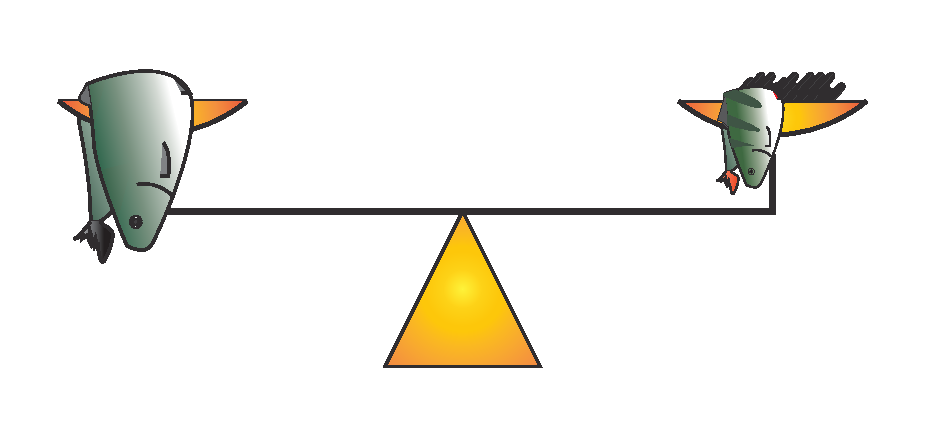
\includegraphics[scale=0.6]{02-yhtalot/kuvia/Kuva10-1-vaaka.pdf} % CC-BY Lilja Tamminen
 %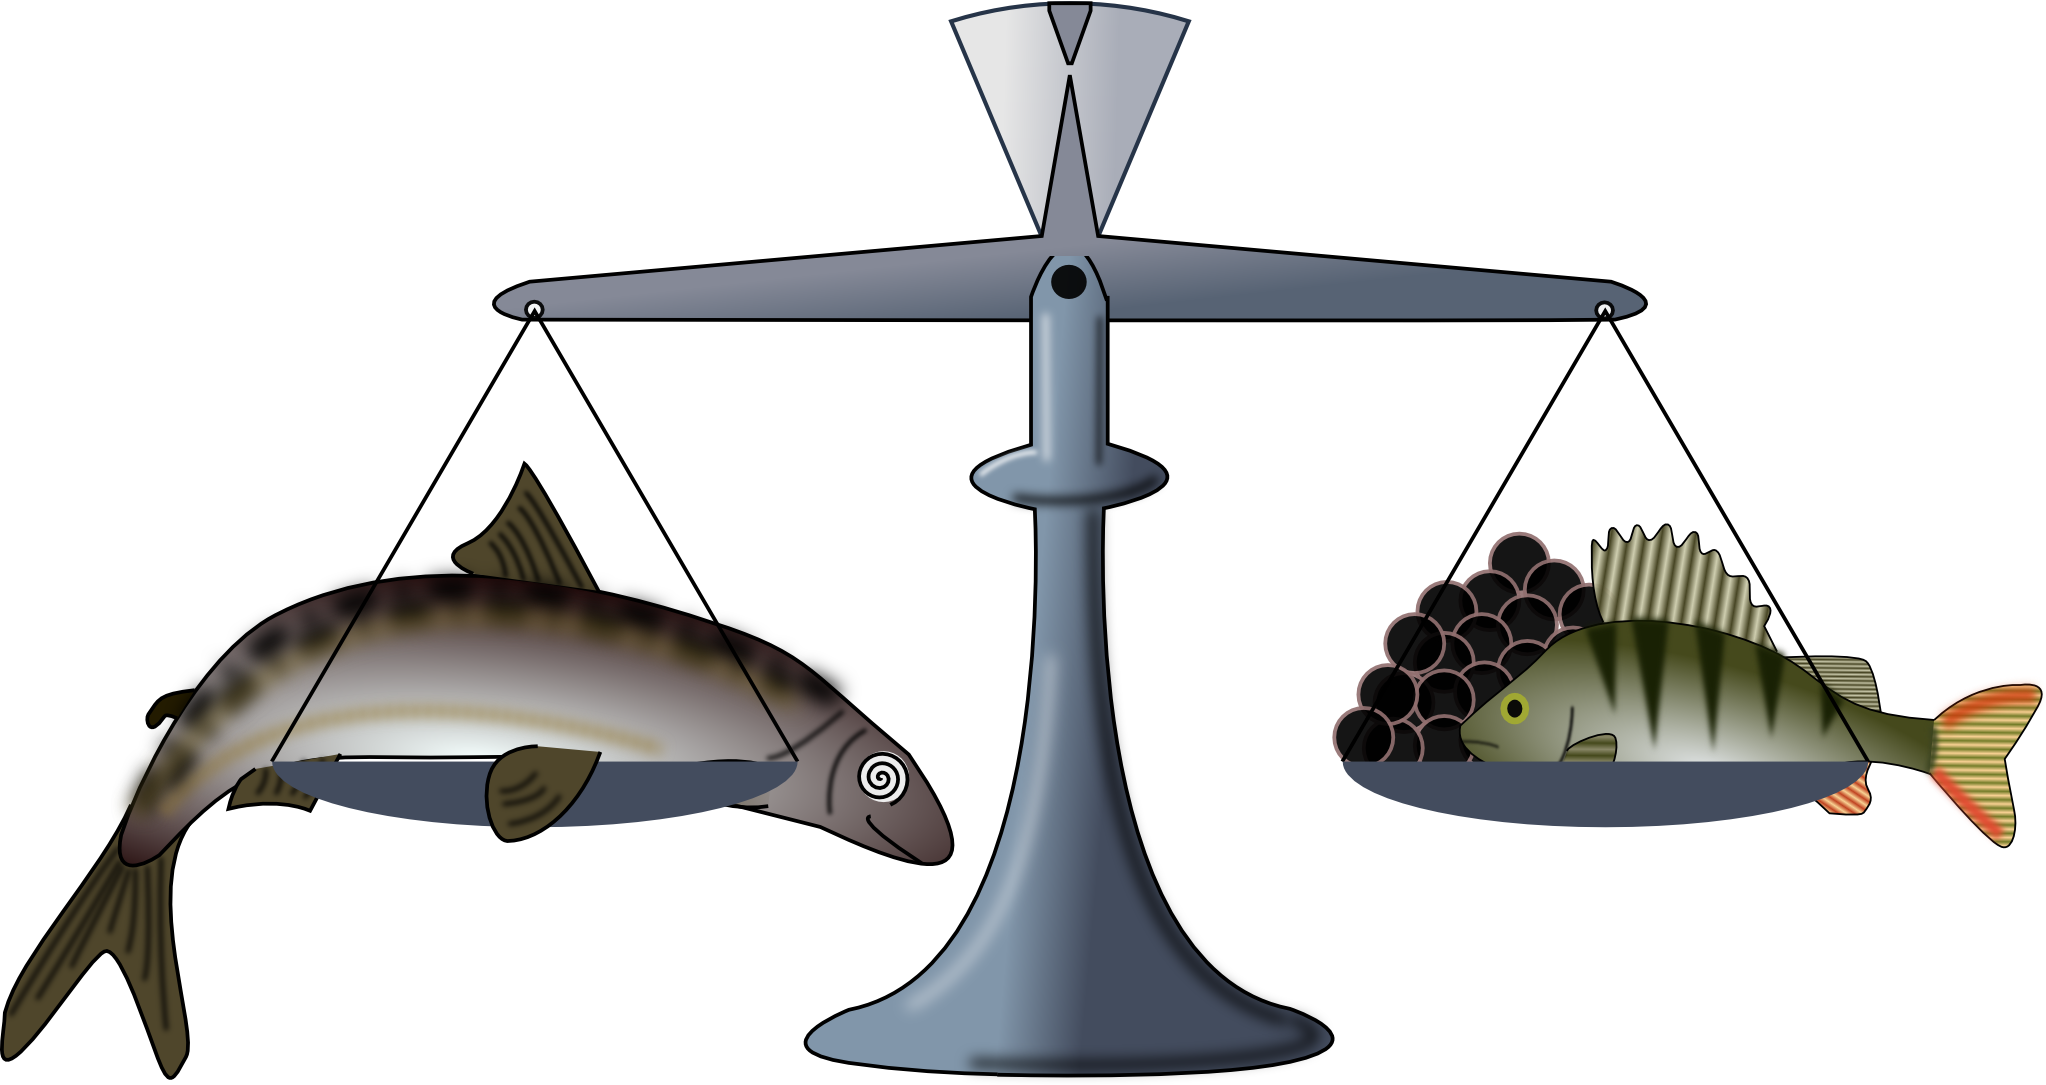
\includegraphics{02-yhtalot/kuvia/kala-vaaka.png} % CC-BY Hannu Köngäs
 % FIXME Hannun piirros on viimeistellympi (smoothit värjäykset jne.), Liljan piirros taas konsistentimpi
 % kirjan muun kuvituksen kanssa. Kumpi jätetään? Nyt päällä Liljan kuva.
 \end{center}


\textbf{Ratkaisu.}

Merkitään lakritsin määrää tuntemattomalla $x$. Tilannetta kuvaa yhtälö
\begin{equation*}
2 = 0{,5} + x.
\end{equation*}

Ratkaistaan yhtälö.

\begin{align*}
2 &= 0{,5} + x &&\text{| $-0{,5}$} \\
2 - 0{,5} &= x && \\
1{,5} &= x && \\
x &= 1{,5} && \\
\end{align*}


\textbf{Vastaus.} Lakritsia on $1{,5}$ kg.
\end{esimerkki}

% FIXME \todo{lisää yhtälöesimerkkejä} Laitoin tuon ToDon pois rumentamasta kirjaa.


\laatikko{
\begin{itemize}
\item Yhtälössä esiintyy yleensä \emph{tuntemattomia}, joiden arvoa ei tiedetä ja joita merkitään eri symboleilla. Jos tuntemattomia on vain yksi, sitä merkitään yleensä kirjaimella $x$.
\item Niitä tuntemattoman $x$ arvoja, joilla yhtälö pätee, kutsutaan yhtälön \emph{ratkaisuiksi}.
\item Yhtälön ratkaisemisella tarkoitetaan kaikkien yhtälön ratkaisujen selvittämistä.
\end{itemize}
}

% FIXME  \todo{jokin helposti ymmärrettävä esimerkki tuntemattomista} Laitoin tuon ToDon pois rumentamasta kirjaa.

\laatikko{
Tyypillinen tapa ratkaista yhtälöitä on kirjoittaa ne ilmaistuna toisella tavalla. Käytännössä tämä tarkoittaa niiden muokkaamista siten, ettei alkuperäisen yhtälön paikkansapitävyys muutu. Tällaisia sallittuja muunnoksia ovat esimerkiksi:
\begin{itemize}
\item Yhtälön molemmille puolille voidaan lisätä tai molemmilta puolilta voidaan vähentää luku. Esimerkiksi yhtälö $3x+5 = 3$ saadaan näin muotoon $3x = -2$.
\item Yhtälön molemmat puolet voidaan kertoa nollasta poikkeavalla luvulla.
Esimerkiksi kertomalla yhtälön $2x = 4$ molemmat puolet luvulla $\frac{1}{2}$
saadaan yhtälö $x = 2$.
\end{itemize}
}

Kuvitellaan orsivaaka, joka on tasapainossa. Vasemmalla ja oikealla puolella on eripainoisia esineitä, mutta ne painavat yhteensä yhtä paljon. Jos molemmille puolille lisätään nyt saman verran painoa, vaaka on yhä tasapainossa. Samalla tavalla yhtälön molemmille puolille on sallittua lisätä sama luku.

Yhtälöt ratkeavat siten, että niitä muokataan, kunnes vastauksen voi lukea siitä suoraan, esim $x=3$.
%Koska jokaisessa muokkausjonon yhtälössä ratkaisut ovat samat, näin saadaan %alkuperäisen yhtälön ratkaisut.

%%esimerkki tulee 1. asteen yhtälön yhteydessä

\laatikko{
Yhtälöitä on kolmenlaisia:
\begin{enumerate}
\item Yhtälö, joka on aina tosi. Esimerkiksi yhtälöt $8=8$ ja $x=x$.
\item Yhtälö, joka on joskus tosi. Esimerkiksi yhtälö $x+4=7$ on tosi, kun $x=3$,
ja epätosi muulloin.
\item Yhtälö, joka ei ole koskaan tosi. Esimerkiksi yhtälö $0=1$.
\end{enumerate}
}

Tärkeimpiä näistä ovat joskus todet yhtälöt.

\laatikko{Yleisiä yhtälönratkaisuperiaatteita:

\begin{itemize}
\item Kerro tuntematonta sisältävät lausekkeet pois nimittäjistä.
\item Yhdistä useat murtolausekkeet yhdeksi laventamalla.
\item Yhdistä tuntemattomat.
\item Kumoa juuret korottamalla yhtälö puolittain sopivaan potenssiin.
\item Sulkuja ei välttämättä aina kannata kertoa auki.
\item Yhtälö on ratkaistu vasta, kun jäljellä on enää vain yksi kappale tuntematonta suuretta, ja se sijaitsee yksin omalla puolellaan yhtälöä.


\end{itemize}
}

Siirrymme nyt tarkastelemaan tärkeää yhtälöiden lajia, ensimmäisen asteen yhtälöitä.
